\documentclass[a4paper, 12pt]{article}
\usepackage[spanish]{babel}
\usepackage[utf8]{inputenc}
\usepackage{amsmath}
\usepackage{indentfirst}
\usepackage{graphicx}
\usepackage[colorinlistoftodos]{todonotes}
\usepackage{esint}
\usepackage{multicol}
\usepackage{listings}
\usepackage{xcolor}

\definecolor{codegreen}{rgb}{0,0.6,0}
\definecolor{codegray}{rgb}{0.5,0.5,0.5}
\definecolor{codepurple}{rgb}{0.58,0,0.82}
\definecolor{backcolour}{rgb}{0.95,0.95,0.92}

\lstdefinestyle{customc}{
	language=C,
    backgroundcolor=\color{backcolour},   
    commentstyle=\color{codegreen},
    keywordstyle=\color{magenta},
    numberstyle=\tiny\color{codegray},
    stringstyle=\color{codepurple},
    basicstyle=\ttfamily\footnotesize,
    breakatwhitespace=false,         
    breaklines=true,                 
    captionpos=b,                    
    keepspaces=true,                 
    numbers=left,                    
    numbersep=5pt,                  
    showspaces=false,                
    showstringspaces=false,
    showtabs=false,                  
    tabsize=2
}

\lstdefinestyle{customasm}{
	language=[x86masm]Assembler,
    backgroundcolor=\color{backcolour},   
    commentstyle=\color{codegreen},
    keywordstyle=\color{magenta},
    numberstyle=\tiny\color{codegray},
    stringstyle=\color{codepurple},
    basicstyle=\ttfamily\footnotesize,
    breakatwhitespace=false,         
    breaklines=true,                 
    captionpos=b,                    
    keepspaces=true,                 
    numbers=left,                    
    numbersep=5pt,                  
    showspaces=false,                
    showstringspaces=false,
    showtabs=false,                  
    tabsize=2
}

\lstset{escapechar=@,style=customasm}

\lstset{literate=
  {á}{{\'a}}1 {é}{{\'e}}1 {í}{{\'i}}1 {ó}{{\'o}}1 {ú}{{\'u}}1
  {Á}{{\'A}}1 {É}{{\'E}}1 {Í}{{\'I}}1 {Ó}{{\'O}}1 {Ú}{{\'U}}1
  {à}{{\`a}}1 {è}{{\`e}}1 {ì}{{\`i}}1 {ò}{{\`o}}1 {ù}{{\`u}}1
  {À}{{\`A}}1 {È}{{\'E}}1 {Ì}{{\`I}}1 {Ò}{{\`O}}1 {Ù}{{\`U}}1
  {ä}{{\"a}}1 {ë}{{\"e}}1 {ï}{{\"i}}1 {ö}{{\"o}}1 {ü}{{\"u}}1
  {Ä}{{\"A}}1 {Ë}{{\"E}}1 {Ï}{{\"I}}1 {Ö}{{\"O}}1 {Ü}{{\"U}}1
  {â}{{\^a}}1 {ê}{{\^e}}1 {î}{{\^i}}1 {ô}{{\^o}}1 {û}{{\^u}}1
  {Â}{{\^A}}1 {Ê}{{\^E}}1 {Î}{{\^I}}1 {Ô}{{\^O}}1 {Û}{{\^U}}1
  {ã}{{\~a}}1 {ẽ}{{\~e}}1 {ĩ}{{\~i}}1 {õ}{{\~o}}1 {ũ}{{\~u}}1
  {Ã}{{\~A}}1 {Ẽ}{{\~E}}1 {Ĩ}{{\~I}}1 {Õ}{{\~O}}1 {Ũ}{{\~U}}1
  {œ}{{\oe}}1 {Œ}{{\OE}}1 {æ}{{\ae}}1 {Æ}{{\AE}}1 {ß}{{\ss}}1
  {ű}{{\H{u}}}1 {Ű}{{\H{U}}}1 {ő}{{\H{o}}}1 {Ő}{{\H{O}}}1
  {ç}{{\c c}}1 {Ç}{{\c C}}1 {ø}{{\o}}1 {å}{{\r a}}1 {Å}{{\r A}}1
  {€}{{\euro}}1 {£}{{\pounds}}1 {«}{{\guillemotleft}}1
  {»}{{\guillemotright}}1 {ñ}{{\~n}}1 {Ñ}{{\~N}}1 {¿}{{?`}}1 {¡}{{!`}}1  {°}{{$^\circ$}}1
}

\setlength{\marginparwidth}{2cm}
\begin{document}
\begin{titlepage}
	\begin{center}
		{\large{UNIVERSIDAD TECNOLÓGICA NACIONAL}}
	\end{center}
	\vspace{15pt}
	\begin{figure}[!ht]
		\centering
		\begin{center}
			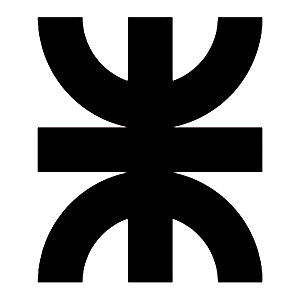
\includegraphics[width=5cm]{utn.png}
		\end{center}
	\end{figure}
	\vspace{5pt}
	\begin{center}
		{\large{FACULTAD REGIONAL PARANÁ}}
		\vspace{5pt}
		\begin{center}
			\vspace{15pt}
			\normalsize{CARRERA: Ingeniería Electrónica\\
						CÁTEDRA: Técnicas Digitales II\\}
			\vspace{50pt}
			\huge\bfseries{Trabajo Práctico N°10\\
			Control de intensidad de LED con PWM\\}
			\vspace{50pt}
		\end{center}
		
		\begin{flushleft}
			\begin{center}
				ALUMNOS:\\
				Battaglia Carlo\\
				Escobar Gabriel\\
			\end{center}
		\end{flushleft}
		
		\begin{center}
			\vspace{\fill}
			\normalsize{Paraná,}
			\today
		\end{center}
	\end{center}
\end{titlepage}

\newpage
\pagenumbering{arabic}
\numberwithin{equation}{section}

Para implementar el sistema requerido, elegimos el \textit{Timer/Counter1} de 16 bits que posee el \textit{ATmega328p} para hacer uso de su función \textit{Fast PWM}.

Configuramos este modo de manera que el ciclo de trabajo de la señal PWM esté dada por el valor almacenado en el registro \textit{OCR1A} y el valor máximo del contador está dado por el registro \textit{ICR1}. Esto nos permite elegir la resolución requerida en el enunciado (16 valores) fijando el máximo en 15 a través de \textit{ICR1}.

Además, para cumplir con la condición de obtener una señal completamente nula al ser el ciclo de trabajo igual a 0, configuramos el modo \textit{Fast PWM} para hacer uso de la señal en modo invertido, tal como se ve en la siguiente tabla:

\begin{center}
	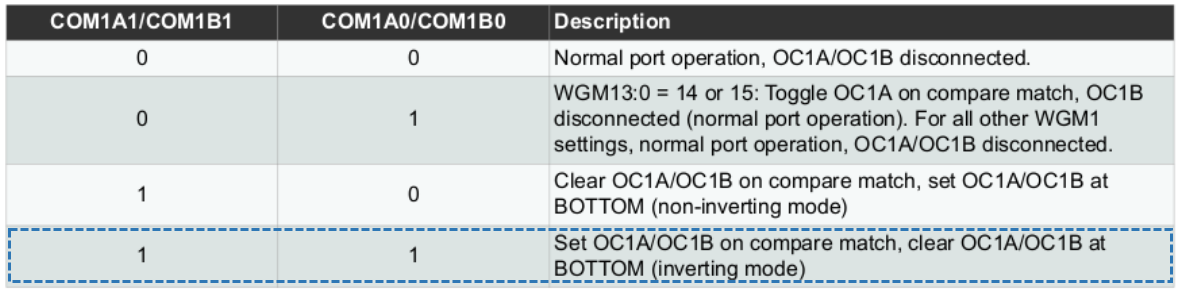
\includegraphics[width=12cm]{tabla.png}
\end{center}

Esto es debido a que en el caso particular en que \textit{OCR1A} es seteado al mismo valor que \textit{BOTTOM (0x0000)} la salida no será una señal nula como habría de esperarse, sino que será un pico angosto con un ancho de un ciclo de timer cada vez que se alcance \textit{TOP+1}.

Al tomar esta decisión de diseño, debimos tener en cuenta que los valores tomados directamente de los pulsadores leyendo el registro \textit{PINC} estarán invertidos a fines prácticos, por lo que han de ser tratados mediante una operación \textit{XOR} con un valor de \textit{0x0F} antes de poder ser cargados en el registro \textit{OCR1A}.

\section{Circuito implementado}

\begin{center}
	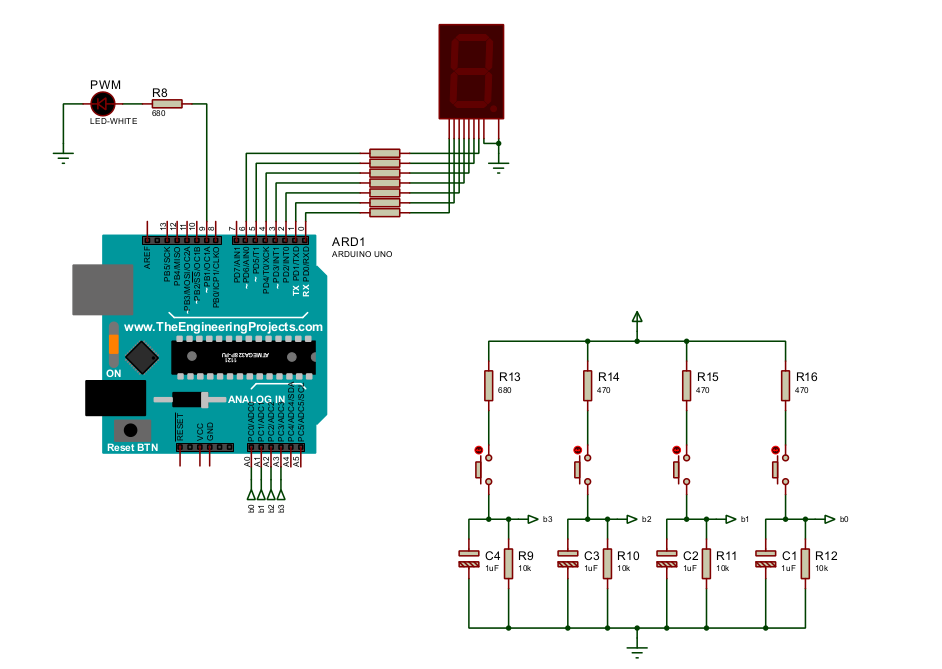
\includegraphics[width=15cm]{circuito.png}
\end{center}

\section{Código}

\small{\lstinputlisting[language={[x86masm]Assembler}]{../main.asm}}
 
\end{document}
